\section{Antrieb}

Im Detroit kann die Geschwindigkeit mittels eines Stufenschalters mit fünf Positionen ausgewählt werden. Um die Funktion des Stufenschalters zu verstehen ist es unabdingbar, zu Beginn einen Blick auf die Funktionsweise des Motors zu richten. Anschliessend werden die verschiedenen Schaltungen, die mit dem Stufenschalter realisierbar sind, vorgestellt.

\subsection{Funktion des Reihenschlussmotores}\label{gm}

Grundsätzlich ist der verwendete Motor ein Gleichstrommotor. Für diesen Motor sind die beiden Gleichungen \ref{eq:motor_dc_i} und \ref{eq:motor_dc_u} ausschlaggebend, welche die Funktion des idealen Ankers beschreiben ($k$ steht dabei für eine Maschinenkonstante, die die Konstruktion des Motors zusammenfasst):
\begin{equation}
	M_{el}=k\cdot\Phi_E\cdot I_A
\label{eq:motor_dc_i}
\end{equation}
\begin{equation}
	U_i=k\cdot\Phi_E\cdot\omega_{me}
\label{eq:motor_dc_u}
\end{equation}
Wichtig ist die Bemerkung, dass diese Gleichungen für den idealen Anker gelten. Bei einem realen Motor addiert sich zur induzierten Spannung $U_i$ noch die Spannung über dem ohmschen Ankerwiderstand $R_A\cdot I_A$. Ausserdem entstehen im Motor selbst Reibungen, die das verfügbare mechanische Drehmoment reduzieren (beispielsweise Lager oder Lüfter).

Wird angenommen, dass die Nichtlinearitäten klein sind im Vergleich zum idealen Modell, kann gesagt werden, dass der Strom proportional zum Moment und die Spannung proportional zur Winkelgeschwindigkeit ist. Mit dem Erregerfluss $\Phi_E$ können dabei beide Grössen beeinflusst werden: \begin{itemize}
	\item Bei erhöhtem Erregerfluss wird das Moment pro Strom grösser, jedoch die Winkelgeschwindigkeit pro Spannung kleiner
	\item Bei verringertem Erregerfluss wird die Winkelgeschwindigkeit pro Spannung grösser, jedoch das Moment pro Strom kleiner
\end{itemize}

Über einen veränderlichen Erregerfluss können also gezielt Moment und Geschwindigkeit aneinander angepasst werden. Genau dieses Verhalten wird im Reihenschlussmotor ausgenutzt. Bevor jedoch auf dessen Funktion eingegangen wird, soll der schematische Aufbau des Reihenschlussmotors in Abbildung \ref{fig:reihenschluss} erläutert werden.

\newpage

\begin{figure}[h!]
	\centering
		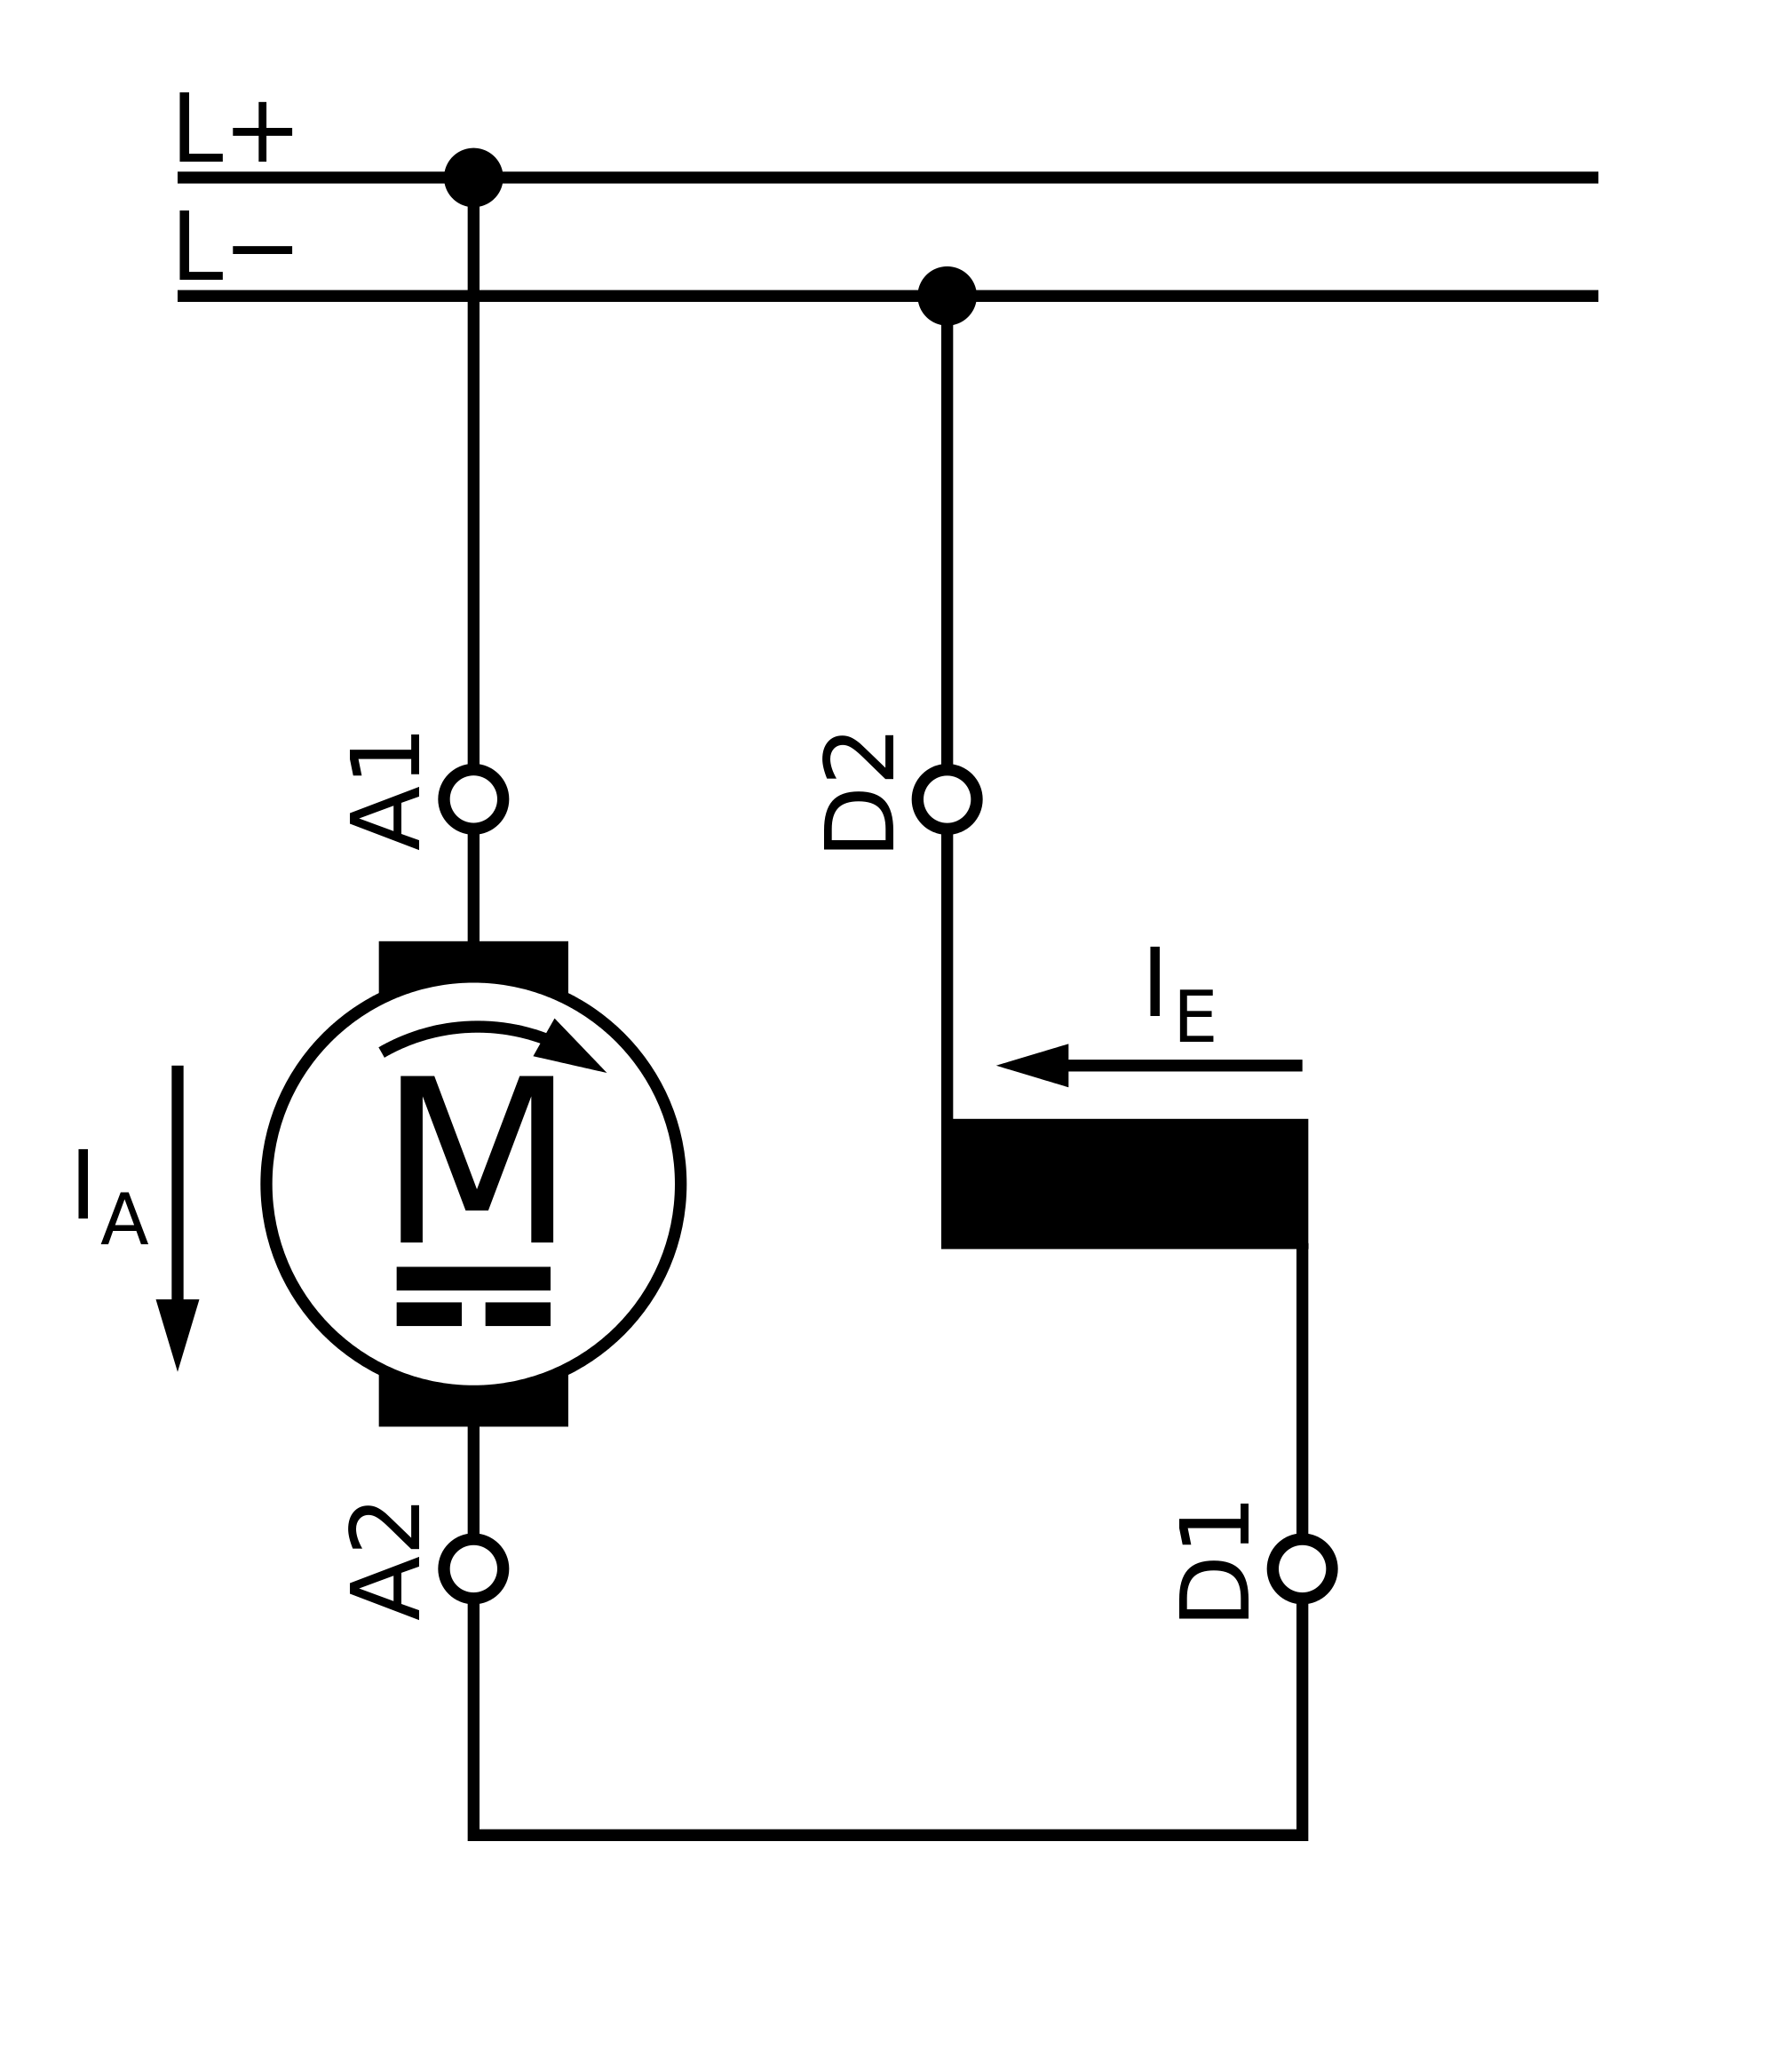
\includegraphics[width=0.45\textwidth]{images/Reihenschlussmotor.png}
	\caption{Elektrisches Schema eines Reihenschlussmotors \cite{wiki_reihenschlussmotor}}
	\label{fig:reihenschluss}
\end{figure}

Der Erregerfluss ist dabei vom Erregerstrom abhängig, wie in Formel \ref{eq:dc_motor_phie} gezeigt ist:
\begin{equation}
	\Phi_E=\frac{L_E}{N_E}\cdot I_E
\label{eq:dc_motor_phie}
\end{equation}\newpage

Da durch Anker und Erregerwicklung der selbe Strom fliesst, somit gilt $I_A=I_E$, sieht man sehr gut, dass bei sinkendem Stromfluss zum einen das Moment aufgrund von Formel \ref{eq:motor_dc_i} kleiner wird, zum anderen das Moment auch durch die schwächere Erregung (aufgrund des geringeren Stromes) kleiner wird. Das Moment ist also quadratisch abhängig vom Stromfluss. Wird ausserdem die weitere Maschinenkonstante $c=k\cdot\frac{L_E}{N_E}$ gesetzt, resultieren für die ideale Reihenschlussmaschine die beiden Formeln \ref{eq:reihenschluss_m} und \ref{eq:reihenschluss_w}:
\begin{equation}
	M_{el}=c\cdot I^2
\label{eq:reihenschluss_m}
\end{equation}
\begin{equation}
	\omega_{me}=\frac{U_i}{c\cdot I}
\label{eq:reihenschluss_w}
\end{equation}
Da auch bei der Reihenschlussmaschine der ohmsche Spannungsabfall über Anker- und Erregerwicklung einen zum Strom proportionalen Spannungsabfall bewirkt, stellt sich für jede angelegte Spannung automatisch ein Gleichgewicht zwischen Drehzahl und Drehmoment ein. Dies erlaubt jedoch weder eine vernünftige Regelung der Geschwindigkeit, noch ist es in jedem möglichen Arbeitspunkt besonders effizient.

Um diese Probleme anzugehen, wird mit der sogenannten Feldschwächung gearbeitet: Bei niedrigen Drehzahlen, wo hohes Moment gefordert ist, wird die Erregung komplett in Serie zum Anker geschaltet. Sind bei höheren Drehzahlen nicht mehr so hohe Momente benötigt, wird ein Teil des Stromes "an der Erregerwicklung vorbei" geleitet, sodass die Erregung zusätzlich geschwächt wird. Dies wird als Feldschwächung bezeichnet.

\subsection{Funktion des Stufenschalters}

Diese Effekte, die beim Reihenschlussmotor bereits vorgestellt wurden, werden vom Stufenschalter gesteuert. Dies ist zum einen die Spannung über dem Motor, zum anderen ist auch eine Feldschwächung möglich. Im Folgenden sollen die fünf Fahrstufen sowie die ursprüngliche Ladestufe vorgestellt werden.

\begin{minipage}{0.49\textwidth}
	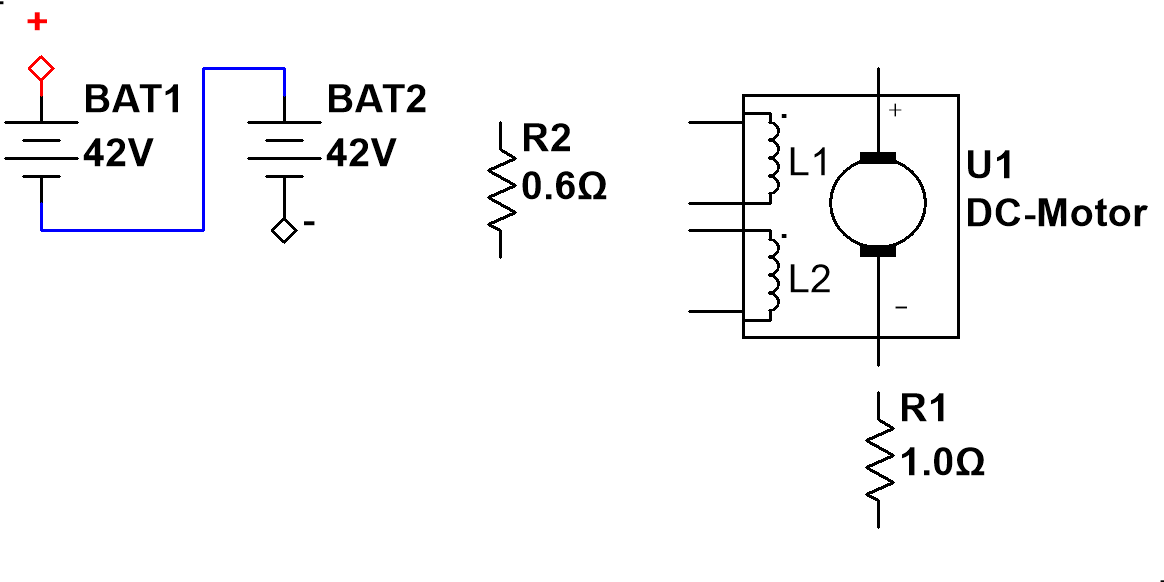
\includegraphics[width=\columnwidth]{images/Stufenschalter/Laden.png}%
\end{minipage}
\begin{minipage}{0.5\textwidth}
	\paragraph{Stufe: Laden}
	In der Nullstellung des Stufenschalters ist die Batterie im Lademodus. Dazu sind beide Batterien in Serie geschalten, sodass beide Batterien mit dem selben Strom geladen werden. Sämtliche Komponenten des Motors sowie die beiden Widerstände sind nicht angeschlossen. Diese Stufe ist auch nach dem Umbau des Detroits weiterhin vorhanden. Das serielle Laden der beiden Batterien wird aber durch die verbauten Dioden verhindert.
\end{minipage}

\begin{minipage}{0.49\textwidth}
	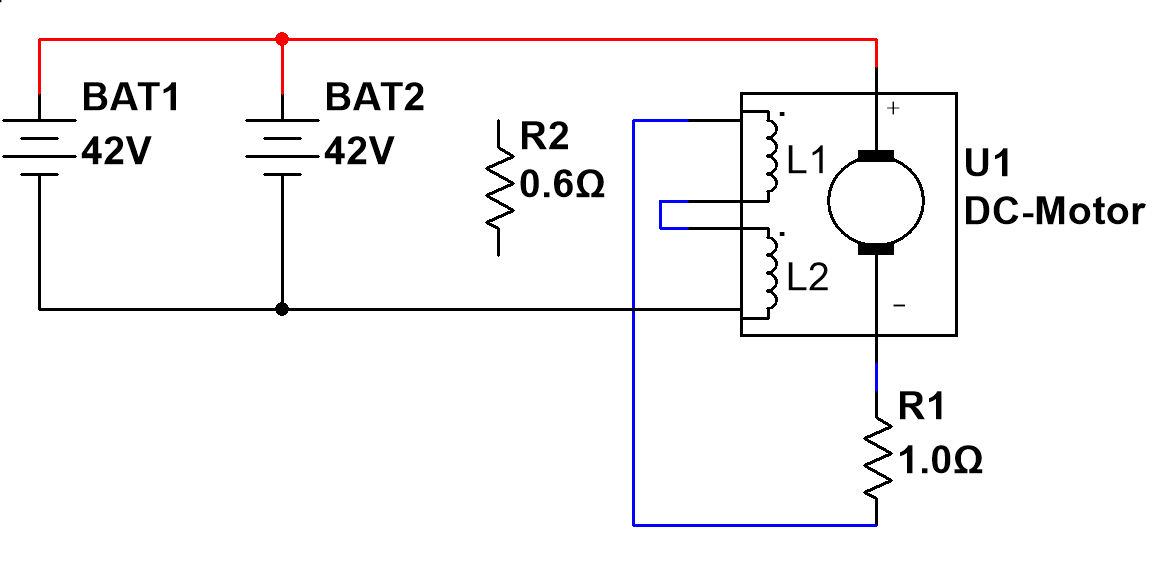
\includegraphics[width=\columnwidth]{images/Stufenschalter/Stufe_1.png}%
\end{minipage}
\begin{minipage}{0.5\textwidth}
	\paragraph{Stufe: Eins}
	In der ersten Fahrstufe werden die beiden Batterien parallel geschaltet, wodurch zum einen die Spannung verringert wird, zum anderen auch der für grosse Momente benötigte Strom geliefert werden kann. Um ein maximales Moment zu erreichen, sind beide Feldwicklungen in Serie angeschlossen, wodurch durch beide der volle Fahrstrom fliesst. Ausserdem ist zur Begrenzung des Anlaufstromes (da im ersten Moment die induzierte Spannung $U_i=0V$ beträgt) der Widerstand $R_1$ in Serie geschaltet.
\end{minipage}

\begin{minipage}{0.49\textwidth}
	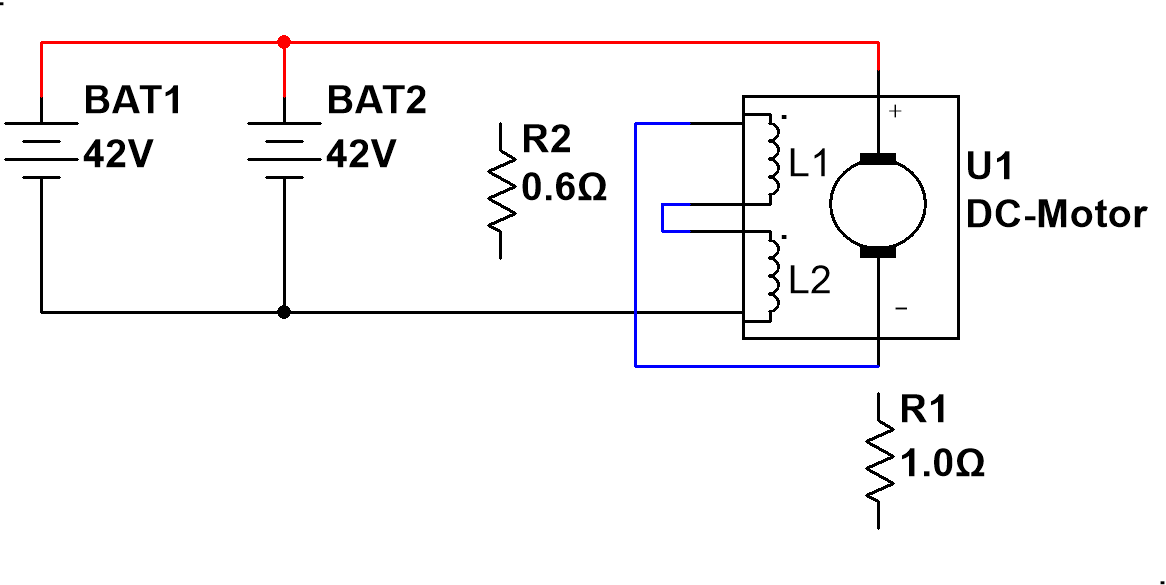
\includegraphics[width=\columnwidth]{images/Stufenschalter/Stufe_2.png}%
\end{minipage}
\begin{minipage}{0.5\textwidth}
	\paragraph{Stufe: Zwei}
	Die zweite Stufe ist fast gleich aufgebaut wie die erste. Auch hier wird für ein möglichst grosses Moment die Serieschaltung der Erregerwicklungen sowie die Parallelschaltung der Batterien verwendet. Der einzige Unterschied zur ersten Fahrstufe ist, dass der Anfahrwiderstand $R_1$ überbrückt und somit funktionslos ist. Durch den weggefallenen Spannungsabfall über dem Anfahrwiderstand wird die erreichbare induzierte Spannung grösser, ohne dabei das erreichbare Moment zu reduzieren.
\end{minipage}

\begin{minipage}{0.49\textwidth}
	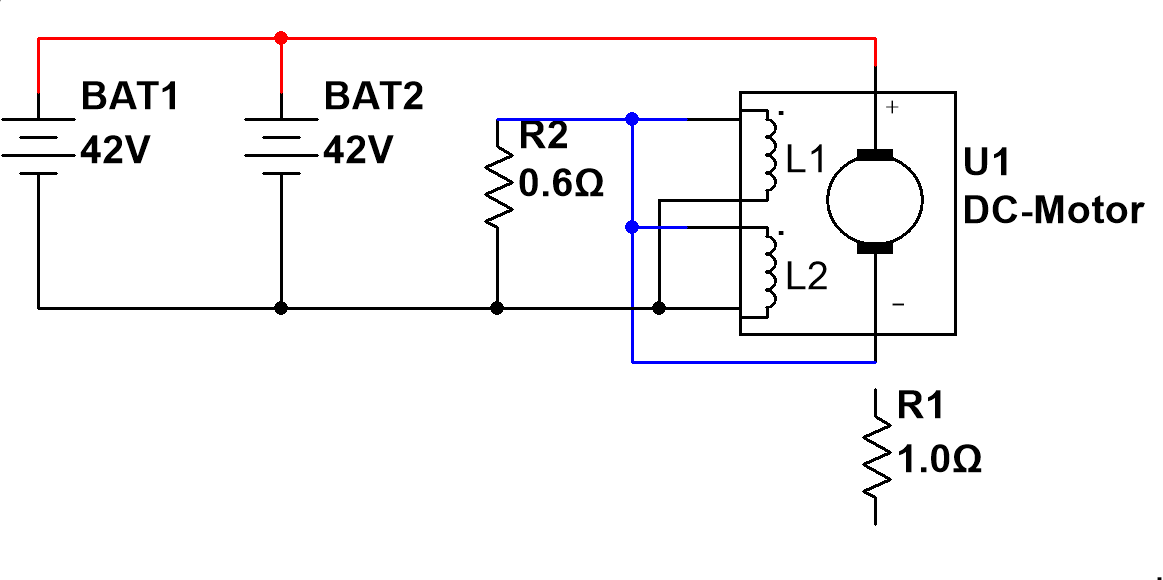
\includegraphics[width=\columnwidth]{images/Stufenschalter/Stufe_3.png}%
\end{minipage}
\begin{minipage}{0.5\textwidth}
	\paragraph{Stufe: Drei}
	In der dritten Stufe wird nun erstmals von der Feldschwächung Gebrauch gemacht. Die beiden Erregerwicklungen sind nicht mehr seriell, sondern parallel geschaltet. Ausserdem ist der Widerstand $R_2$ parallel zu den beiden Erregerwicklungen geschaltet. Durch diese Parallelschaltung ist der Stromfluss in der Erregerwicklung und damit die Erregung selbst deutlich kleiner als in den vorherigen Fahrstufen, wodurch eine höhere Winkelgeschwindigkeit bei reduziertem Moment ermöglicht wird. Die beiden Batterien sind weiterhin parallel geschaltet.
\end{minipage}

\begin{minipage}{0.49\textwidth}
	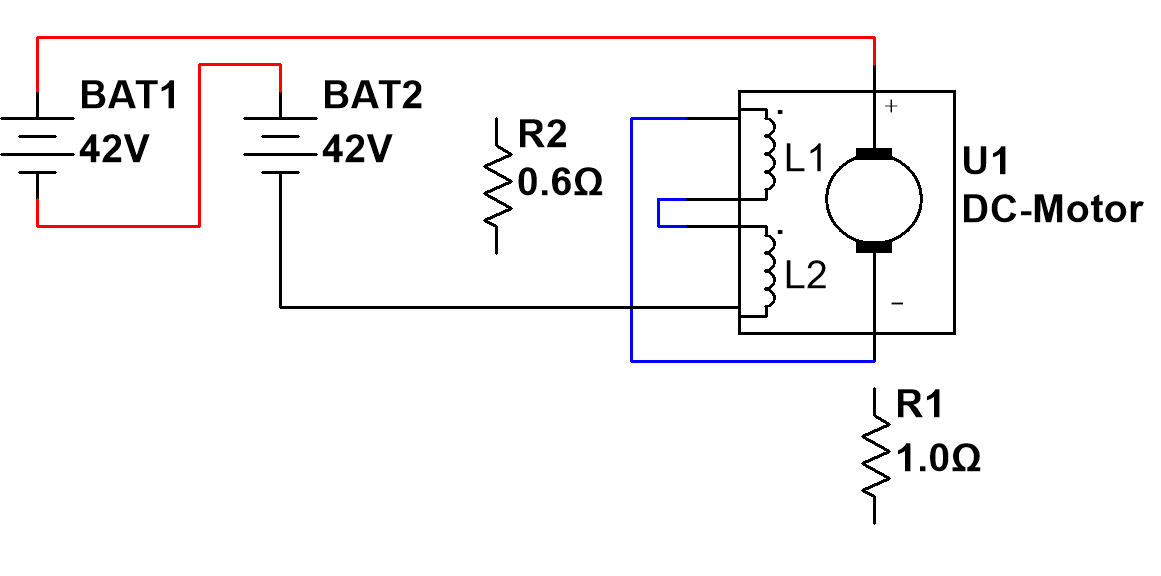
\includegraphics[width=\columnwidth]{images/Stufenschalter/Stufe_4.png}%
\end{minipage}
\begin{minipage}{0.5\textwidth}
	\paragraph{Stufe: Vier}
	In der vierten Fahrstufe wird die Spannung durch Serieschaltung der Batterien erhöht. Um weiterhin grosse Kräfte zu ermöglichen, wird die Erregerwicklung wieder von parallel nach seriell verschaltet, wodurch keine Feldschwächung entsteht. Stufe vier ist deswegen sehr ähnlich aufgebaut wie Stufe zwei, jedoch sind aufgrund der verdoppelten Spannung höhere Leistungen erzielbar als in Stufe zwei. Es ist gut möglich, dass bei den ursprünglichen Blei-Batterien dieser Leistungszuwachs bei hohen Strömen durch den Innenwiderstand der Batterien zum Teil wieder ausgeglichen wurde. Bei den modernen Lithium-Ionen-Akkumulatoren kann dies jedoch dementiert werden. Es ist zudem aufgrund der hohen Spannung und des gleichzeitig starken Feldes zu vermuten, dass in dieser Stufe die grössten Momente entwickelt werden konnten.
\end{minipage}

\begin{minipage}{0.49\textwidth}
	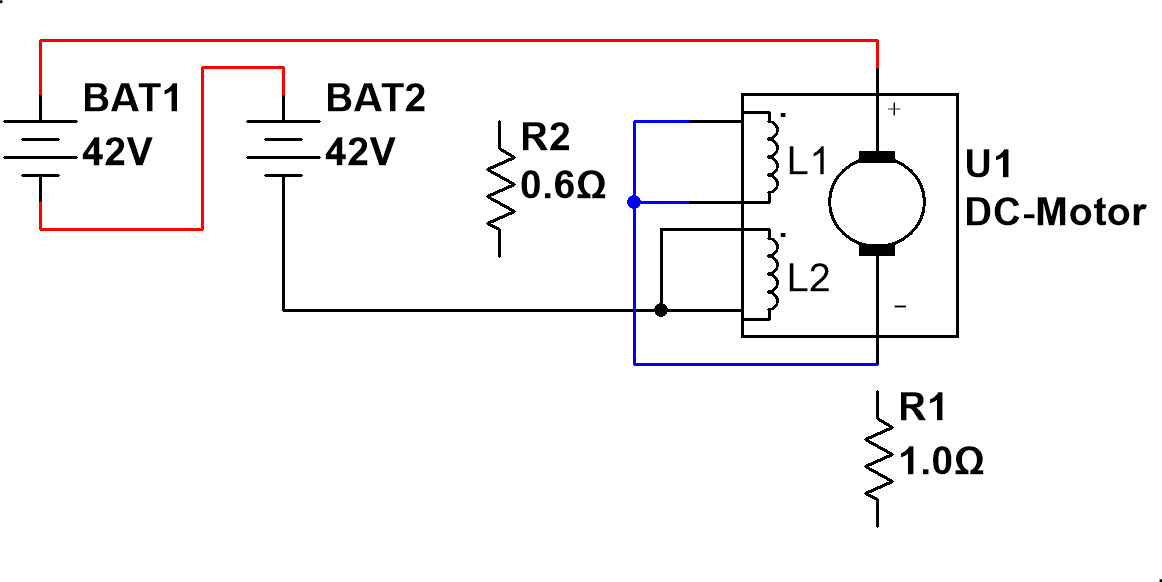
\includegraphics[width=\columnwidth]{images/Stufenschalter/Stufe_5.png}%
\end{minipage}
\begin{minipage}{0.5\textwidth}
	\paragraph{Stufe: Fünf}
	Auch in der fünften und damit höchsten Fahrstufe sind die beiden Batterien für eine höhere Spannung in Serie geschaltet. Hier wird wieder Gebrauch von der Feldschwächung gemacht, indem die beiden Erregerwicklungen parallel geschalten werden und damit der Fluss reduziert wird. Im Gegensatz zur Stufe drei, bei welcher die Erregerwicklungen ebenfalls parallel geschaltet werden, wird hier auf die zusätzliche Parallelschaltung des Widerstandes $R_2$ und damit auf die weitere Reduktion des Feldes verzichtet. Dadurch sollten sich auch noch bei hohen Geschwindigkeiten genügende Momente ergeben.
\end{minipage}

Die Fahrstufen werden dabei vom Stufenschalter mechanisch geschaltet, indem unter den Kontaktfingern mittels Kupferplatten Kontakte verbunden (und damit beispielsweise Widerstände überbrückt) werden. Die Lagen dieser Kupferplatten ist im Originalschema zu finden, wie es im Anhang unter \ref{schema_original} zu finden ist. Ausserdem ist ein Blick in das Innere des Stufenschalters in Abbildung \ref{fig:Stufenschalter} gegeben:

\begin{figure}[h]
	\centering
		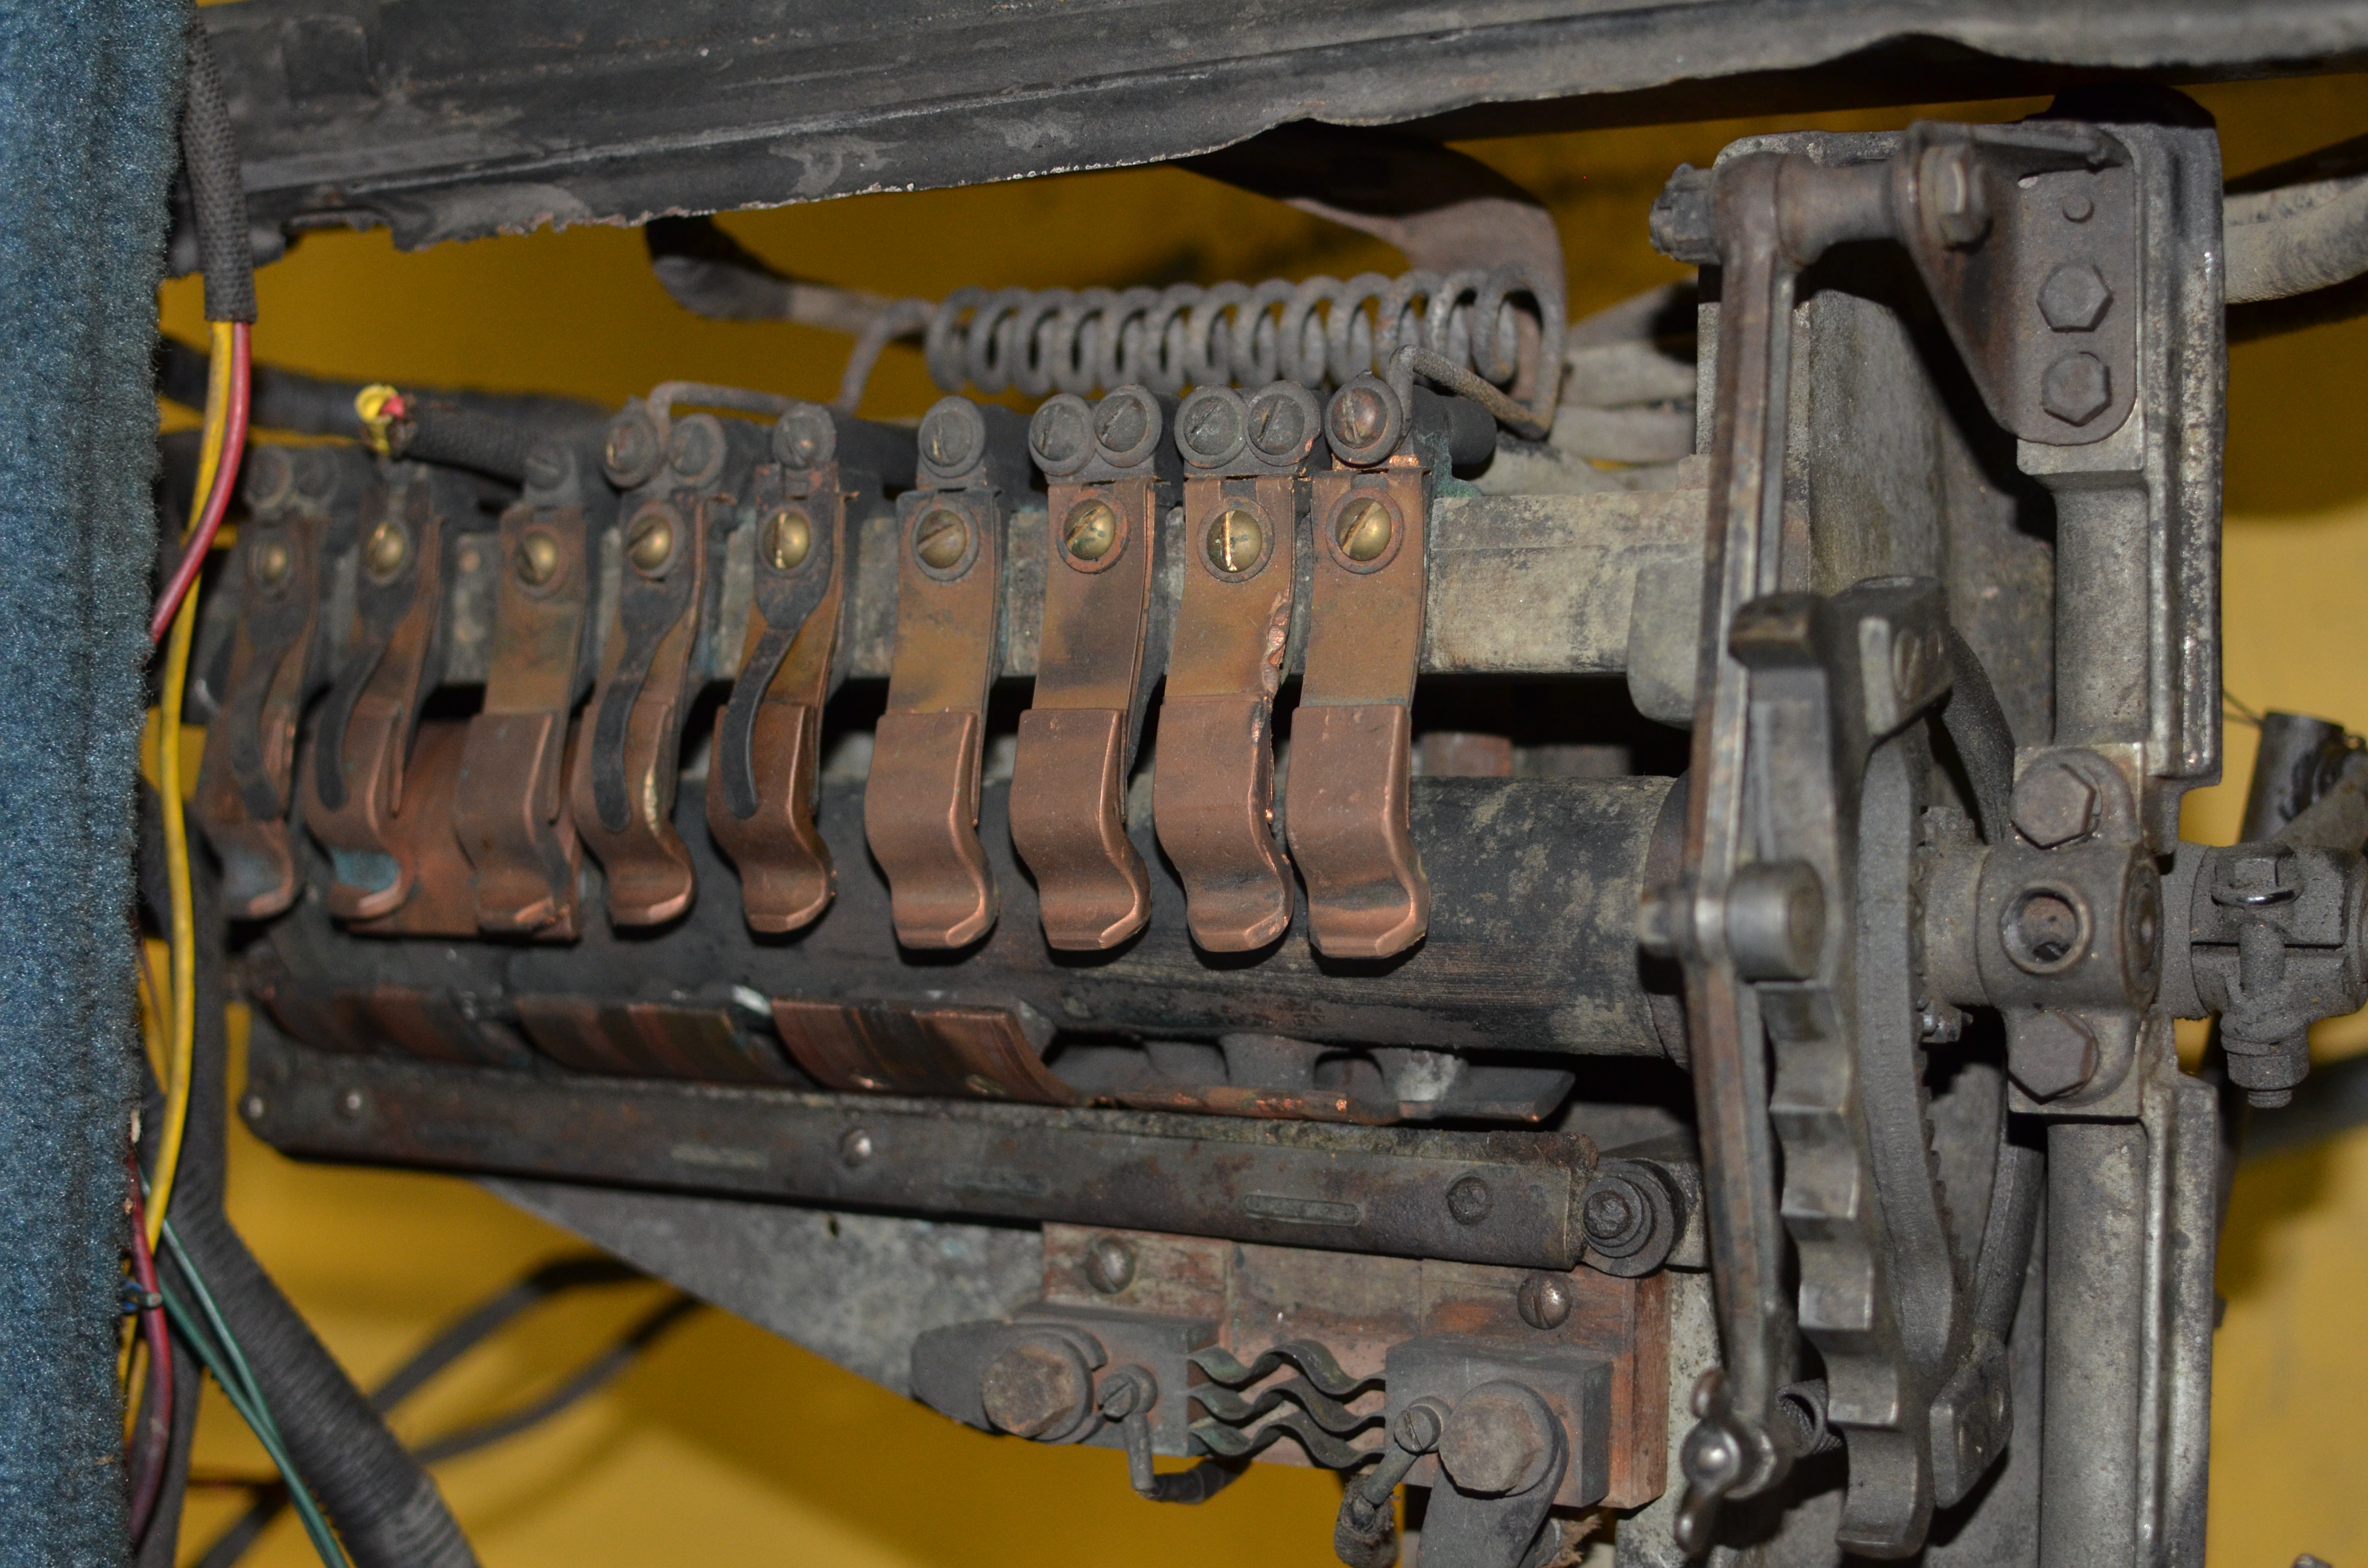
\includegraphics[width=0.8\textwidth]{images/Stufenschalter/Foto}
	\caption{Blick in den geöffneten Stufenschalter}
	\label{fig:Stufenschalter}
\end{figure}

Glücklicherweise befand sich der Stufenschalter in einem guten Zustand, sodass lediglich etwas Staub entfernt werden musste. Ausserdem wurde ein Teil der Verkabelung erneuert, sodass diese ebenfalls am Stufenschalter befestigt werden konnte.

\newpage